\chapter{Pooling}

A standard layer in a convolutional network is typically composed of three stages. First, multiple convolutions are applied in parallel to generate linear activations. Next, these activations are passed through a nonlinear activation function, a step sometimes referred to as the \textit{detector stage}. Finally, a \textit{pooling operation} is applied to further transform and condense the output.

\begin{figure}[H]
    \centering
    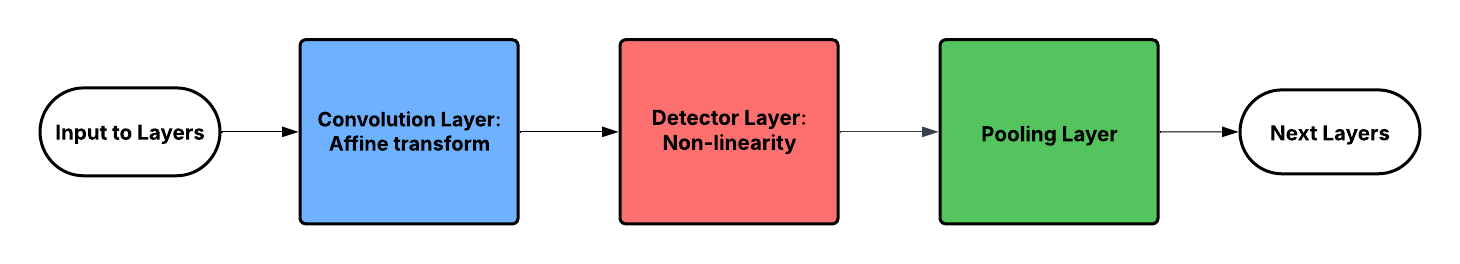
\includegraphics[width=0.7\linewidth]{Images/Chapters/layers.png}
    \caption{Data flow through a typical CNN block.}
    \label{fig:cnn_block_flow}
\end{figure}

Pooling is a subsampling operation that has traditionally played a central role in CNNs.  
Its purpose is to reduce the spatial resolution of feature maps while retaining the most important information. The use of pooling can be viewed as adding an infinitely strong prior that the function the layer learns must be invariant to small translations. When this assumption is correct, it can greatly improve the statistical efficiency of the network \cite{goodfellow2016deep}.
However, when the assumption does not hold, convolution and pooling may actually harm performance. 
Like any prior, these operations are only beneficial when their underlying assumptions are accurate: if a task requires preserving precise spatial information, excessive pooling can increase training error and lead to underfitting. 
For this reason, some architectures apply pooling selectively, on certain channels but not others, to balance the extraction of invariant features with the preservation of fine-grained spatial details.

\section{Definition}

Given an input feature map $X \in \mathbb{R}^{m \times n}$, pooling partitions $X$ into non-overlapping regions and summarizes each region by a statistic.  
The two most common pooling operations are:  

\begin{itemize}
    \item \textbf{Max pooling}, which reports the maximum value within a rectangular \newline neighborhood:
    \begin{equation}
    Y[i,j] = \max_{(p,q) \in \mathcal{R}_{ij}} X[p,q],
    \end{equation}

    \item \textbf{Average pooling}, which computes the mean value:
    \begin{equation}
    Y[i,j] = \frac{1}{|\mathcal{R}_{ij}|} \sum_{(p,q) \in \mathcal{R}_{ij}} X[p,q],
    \end{equation}
\end{itemize}

where $\mathcal{R}_{ij}$ denotes the receptive field corresponding to output element $(i,j)$.  


\section{Motivation and role in CNNs}

The central benefit introduced by pooling lies in the approximately \textbf{invariance to small translations} of the input.

Both max pooling and average pooling summarize local neighbourhoods in a way that makes the representation less sensitive to small shifts in the input.  
This invariance is particularly valuable in visual recognition tasks, when we care more about whether some feature is present than exactly where it is. For example, when recognizing whether an image contains a car, the network does not need to know the exact pixel-level positions of the wheels; it is enough to detect that there are four wheels, with two in the front and two in the back, regardless of small variations in their precise location.

\clearpage

It's also possible, if pooling over the output of separately parametrized convolutions, to make features able to learn \textit{which} transformations to become invariant to.

\begin{figure} [H]
    \centering
    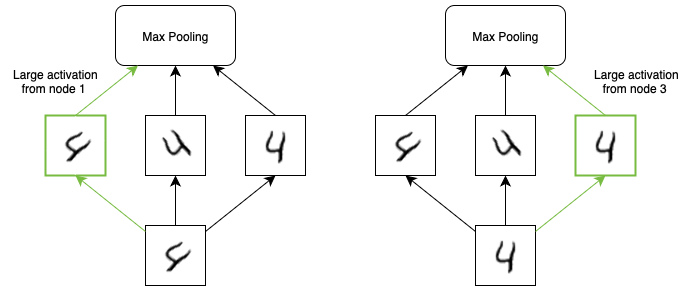
\includegraphics[width=0.7\linewidth]{Images/Chapters/pooling_invariance.png}
    \caption{Example of filters that learn to become invariant to rotation.}
    \label{fig:pooling_invariance}
\end{figure}

Pooling also introduces several important benefits: reduces the spatial resolution of feature maps, which decreases the computational cost of subsequent layers, lowers memory requirements and improves the statistical efficiency of the network by enforcing more compact and robust representations.  

Within the hierarchy of a CNN, pooling therefore plays a key role: early convolutional layers detect local features such as edges, and pooling combines them into progressively more abstract and stable patterns, supporting the network in building higher-level representations \cite{goodfellow2016deep}.


\section{Modern alternatives}
\label{sec:pooling-alternatives}%

While max and average pooling have been widely used, more recent research has explored alternatives that either replace pooling entirely or refine it.  

Springenberg et al., 2015 \cite{springenberg2015allcnn} investigated whether pooling is truly necessary for state of the art performance. They proposed an extremely simple architecture consisting only of convolutional layers, with dimensionality reduction achieved exclusively by \textbf{strided convolutions} (stride of 2).  
Despite the absence of pooling, normalization layers or complex activation functions, this homogeneous architecture was able to achieve competitive, and in some cases state of the art, performance on benchmark datasets such as CIFAR-10, CIFAR-100, ImageNet.   Their findings demonstrated that small convolutional layers with stride can be sufficient to replace traditional pooling operators and raises important questions about the necessity of pooling in CNNs.
 
Traditional pooling operations either discard information (max pooling) or average it uniformly (average pooling), both of which may lead to a loss of useful detail.  
\textbf{SoftPool} (Stergiou et al., 2021 \cite{stergiou2021softpool}) addresses this limitation by computing a weighted average, where the weights are proportional to the magnitude of the activations within each pooling region.  
This mechanism allows more information to be preserved, while still reducing the spatial resolution of the feature maps. Experimental evaluations have shown that SoftPool improves classification accuracy on benchmarks such as ImageNet, CIFAR, and Kinetics, while introducing only minimal computational overhead.  
These results suggest that more informative pooling operators can provide benefits over max and average pooling and highlight the potential of adaptive downsampling methods in modern CNNs.